%------------------------------------------------------------------------------%

\usepackage{calculo_varias_variaveis-1}

\usepackage{tikz}
\usetikzlibrary{angles}

\title {Coordenadas Cartesianas e Polares}

%------------------------------------------------------------------------------%
\begin{document}

\addtitle

%------------------------------------------------------------------------------%
\section{Sistema de Coordenadas Cartesianas}

%------------------------------------------------------------------------------%
\begin{frame}{Sistema de Coordenadas Cartesianas}
  \begin{enumerate}[<+->]
    \item Cada ponto do plano é associado a um par de números reais $(x, y)$
    \item Cada ``figura'' no plano corresponde a um subconjunto de $\R^2$
    \item Na orientação convencional, $x$ aponta para a direita e $y$ para cima
  \end{enumerate}
\end{frame}

%------------------------------------------------------------------------------%
\begin{frame}{Sistema de Coordenadas Cartesianas}
  \centering
  \input{plano_cartesiano}
\end{frame}

%------------------------------------------------------------------------------%
\begin{frame}{Gráfico de uma Função Real}
  Conjunto de pontos $(x, y) \in \R^2$ tais que \(y = f(x)\)

  \pause
  \vspace{\baselineskip}
  Para cada $x$, no domínio, existe \emph{um único} $y$
\end{frame}

%------------------------------------------------------------------------------%
\begin{frame}{Gráfico de uma Função Real}
  \centering
  

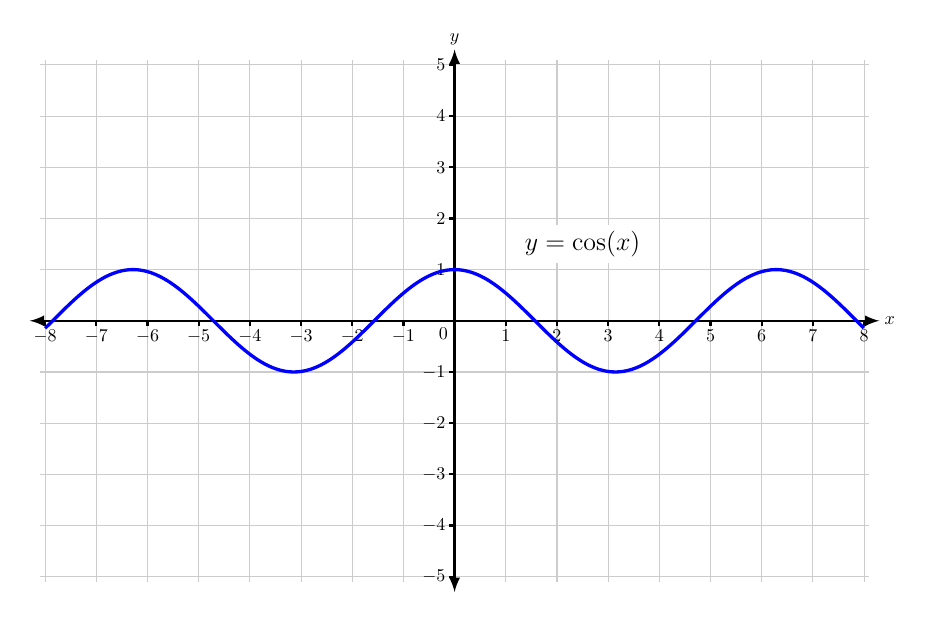
\begin{tikzpicture}[thick,scale=0.65, every node/.style={scale=0.65}]
  \def \minx {-8}
  \def \maxx {8}
  \def \miny {-5}
  \def \maxy {5}

  \draw[thin,black!20] (\minx-0.1,\miny-0.1) grid (\maxx+0.1,\maxy+0.1);

  \draw[thick, latex-latex] (\minx-0.3,0)--(\maxx+0.3,0);
  \draw[thick, latex-latex] (0,\miny-0.3)--(0,\maxy+0.3);
  \node at (\maxx+0.5,0) {$x$};
  \node at (0,\maxy+0.5) {$y$};

  \foreach \x in {\minx,...,-1}{
    \draw (\x,0)--(\x,-0.1);
    \node[below,black] at (\x,-0.05) {$\x$};
  }
  \foreach \x in {1,...,\maxx}{
    \draw (\x,0)--(\x,-0.1);
    \node[below,black] at (\x,-0.05) {$\x$};
  }
  \foreach \y in {\miny,...,-1}{
    \draw (0,\y)--(-0.1,\y);
    \node[left,black] at (-0.05,\y) {$\y$};
  }
  \foreach \y in {1,...,\maxy}{
    \draw (0,\y)--(-0.1,\y);
    \node[left,black] at (-0.05,\y) {$\y$};
  }
  \node[below left,black] at (0,0) {$0$};

  \draw[very thick, domain=\minx:\maxx, variable=\x, smooth, samples=300, blue]  plot ({\x},{cos(\x r)});

  \node at (2.5,1.5) [fill=white] {\Large $y=\cos(x)$};
\end{tikzpicture}

\end{frame}

%------------------------------------------------------------------------------%
\begin{frame}{Soluções de uma Equação}

  Qualquer expressão da forma
  \[
    G(x, y) = 0
  \]

  \pause
  \vspace{\baselineskip}
  Queremos \emph{todos os pares} $(x, y)$ que satisfazem a equação

  \pause
  \vspace{\baselineskip}
  Se faltar um, a solução está incompleta e portanto errada
\end{frame}

%------------------------------------------------------------------------------%
\begin{frame}{Soluções de uma Equação}
  \centering
  \input{grafico_equacao}
\end{frame}

%------------------------------------------------------------------------------%
\begin{frame}{Curvas Paramétricas}
  Funções de $\R$ em $\R^n$
  \[
    \left(\begin{array}{>{\,}c<{\,}}
      x \\[1mm]
      y
    \end{array}\right)
    =
    \left(\begin{array}{>{\,}c<{\,}}
      f(t) \\[1mm]
      g(t)
    \end{array}\right)
  \]

  \pause
  \vspace{\baselineskip}
  Podemos pensar na variável como o tempo e a curva como uma
  trajetória

\end{frame}

%------------------------------------------------------------------------------%
\begin{frame}{Curvas Paramétricas}
  \centering
  

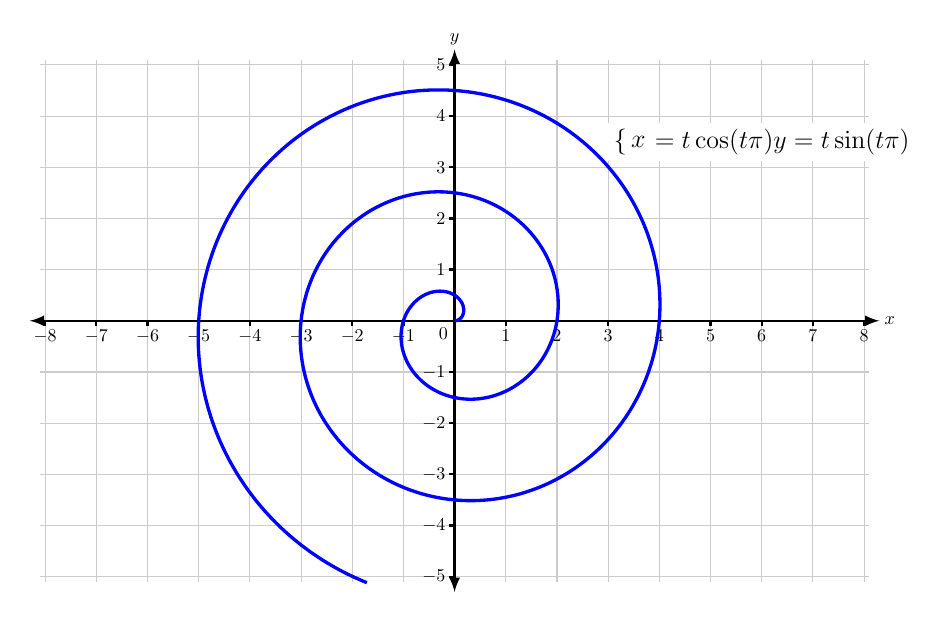
\begin{tikzpicture}[thick,scale=0.65, every node/.style={scale=0.65}]
  \def \minx {-8}
  \def \maxx {8}
  \def \miny {-5}
  \def \maxy {5}

  \draw[thin,black!20] (\minx-0.1,\miny-0.1) grid (\maxx+0.1,\maxy+0.1);

  \draw[thick, latex-latex] (\minx-0.3,0)--(\maxx+0.3,0);
  \draw[thick, latex-latex] (0,\miny-0.3)--(0,\maxy+0.3);
  \node at (\maxx+0.5,0) {$x$};
  \node at (0,\maxy+0.5) {$y$};

  \foreach \x in {\minx,...,-1}{
    \draw (\x,0)--(\x,-0.1);
    \node[below,black] at (\x,-0.05) {$\x$};
  }
  \foreach \x in {1,...,\maxx}{
    \draw (\x,0)--(\x,-0.1);
    \node[below,black] at (\x,-0.05) {$\x$};
  }
  \foreach \y in {\miny,...,-1}{
    \draw (0,\y)--(-0.1,\y);
    \node[left,black] at (-0.05,\y) {$\y$};
  }
  \foreach \y in {1,...,\maxy}{
    \draw (0,\y)--(-0.1,\y);
    \node[left,black] at (-0.05,\y) {$\y$};
  }
  \node[below left,black] at (0,0) {$0$};

  \draw[
    very thick,
    domain=0:5.4,
    variable=\t,
    smooth,
    samples=300,
    blue]
    plot ({\t*cos(\t*3.1415 r)},{\t*sin(\t*3.1415 r)});

  \node at (6,3.5) [fill=white]
  {
      \Large
      $
      \begin{cases}
        x = t \cos(t\pi) \\
        y = t \sin(t\pi)
      \end{cases}
      $
  };
\end{tikzpicture}

\end{frame}

%------------------------------------------------------------------------------%
\begin{frame}{Desigualdades}
  Desigualdades geralmente representam regiões no plano (ou espaço)
\end{frame}

%------------------------------------------------------------------------------%
\begin{frame}{Desigualdades}
  \centering
  

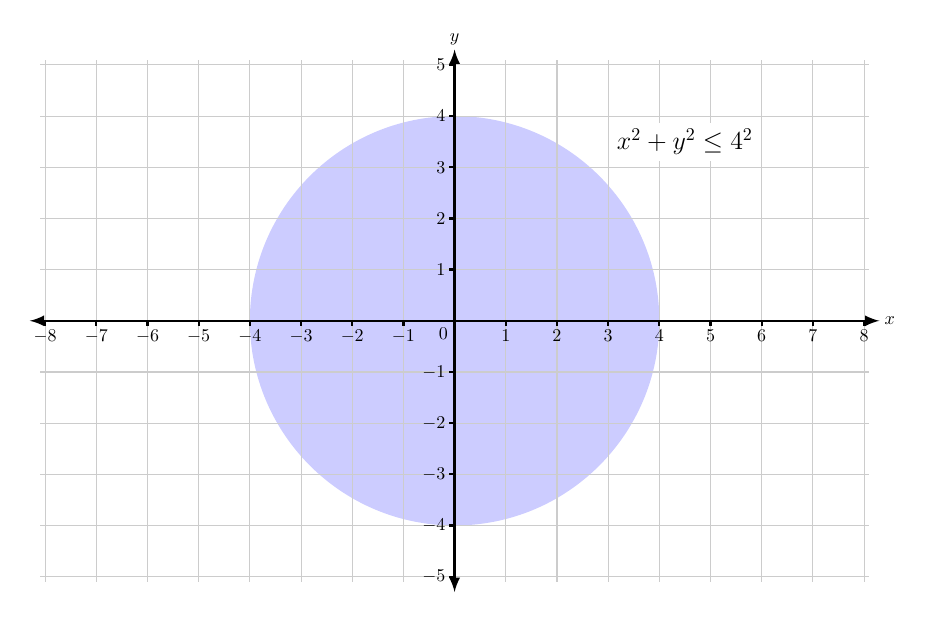
\begin{tikzpicture}[thick,scale=0.65, every node/.style={scale=0.65}]
  \def \minx {-8}
  \def \maxx {8}
  \def \miny {-5}
  \def \maxy {5}

  \fill[fill=blue!20](0,0) circle (4);

  \draw[thin,black!20] (\minx-0.1,\miny-0.1) grid (\maxx+0.1,\maxy+0.1);

  \draw[thick, latex-latex] (\minx-0.3,0)--(\maxx+0.3,0);
  \draw[thick, latex-latex] (0,\miny-0.3)--(0,\maxy+0.3);
  \node at (\maxx+0.5,0) {$x$};
  \node at (0,\maxy+0.5) {$y$};

  \foreach \x in {\minx,...,-1}{
    \draw (\x,0)--(\x,-0.1);
    \node[below,black] at (\x,-0.05) {$\x$};
  }
  \foreach \x in {1,...,\maxx}{
    \draw (\x,0)--(\x,-0.1);
    \node[below,black] at (\x,-0.05) {$\x$};
  }
  \foreach \y in {\miny,...,-1}{
    \draw (0,\y)--(-0.1,\y);
    \node[left,black] at (-0.05,\y) {$\y$};
  }
  \foreach \y in {1,...,\maxy}{
    \draw (0,\y)--(-0.1,\y);
    \node[left,black] at (-0.05,\y) {$\y$};
  }
  \node[below left,black] at (0,0) {$0$};

  \node at (4.5,3.5) [fill=white] {\Large $x^2 + y^2 \leq 4^2$};
\end{tikzpicture}

\end{frame}

%------------------------------------------------------------------------------%
\section{Sistema de Coordenadas Polares}

%------------------------------------------------------------------------------%
\begin{frame}{Coordenadas Polares}
  \centering
  
\begin{tikzpicture}

	% Coordinates
	\coordinate (A) at (6,0);
	\coordinate (B) at (0,0);
	\coordinate (C) at (2.5,2.5);
	\coordinate (B') at (2.5,3.5);
	\coordinate (A') at (1.8,3.2);

	% Axis
	\draw[thick,-latex] (-1ex,0) -- (6,0) node [below] {$x$};
	\draw[thick,-latex] (0,-1ex) -- (0,5) node [left]  {$y$};

	\draw[thick] (0,0) -- (2.5,2.5) node[pos=0.6, above left] {$r$};
  \node at (0.8,0.3) {$\theta$};

	% Help Lines
	\draw[dashed] (0,2.5) -- (2.5,2.5) -- (2.5,0);
	\draw[dashed] (3.53,0) arc (0:90:3.53);

	% Angle
	\pic[draw, ->, thick, angle eccentricity=1.7] {angle = A--B--C};

\end{tikzpicture}

\end{frame}

%------------------------------------------------------------------------------%
\begin{frame}{Coordenadas Polares}
  Definição
  \begin{itemize}[<+->]
    \item Origem ou polo
    \item Raio inicial
    \item $r$ distância orientada até a origem
    \item $\theta$ ângulo orientado a partir do raio inicial (em radianos)
    \item Coordenadas polares $(r, \theta)$
  \end{itemize}
\end{frame}

%------------------------------------------------------------------------------%
\begin{frame}{Equações em Coordenadas Polares}
  \begin{itemize}[<+->]
    \item \(r=a\)              \tabto{16mm} circulo com centro na origem e raio \(\abs{a}\)
    \item \(\theta=\theta_0\)  \tabto{16mm} reta passando pela origem com ângulo $\theta_0$ com o raio inicial
  \end{itemize}
\end{frame}

%------------------------------------------------------------------------------%
\begin{frame}{Relação Entre Coordenadas Polares e Cartesianas}
  \centering
  
\includegraphics[height=68mm]{relacao_polares_catesianas}
\end{frame}

%------------------------------------------------------------------------------%
\begin{frame}{Relação Entre Coordenadas Polares e Cartesianas}
  \[
    x = r\cos(\theta) \qquad\qquad
    y = r\sin(\theta)
  \]

  \pause
  \vspace{\baselineskip}
  \[
    r^2 = x^2 + y^2  \qquad\qquad
    \tan\theta = \frac{x}{y}
  \]
\end{frame}

%------------------------------------------------------------------------------%
\section{Exemplos}

%------------------------------------------------------------------------------%
\begin{frame}{Exemplo 1}
  Encontre todas as coordenadas polares do ponto
  \(
    \left(r,\theta\right) =
    \left(2, \frac{\pi}{6}\right)
  \)

  \pause
  \vspace{\baselineskip}
  Os pares são
  \[
    \left( 2, \frac{\pi}{6}+2n\pi\right)
    \hphantom{--5}
    \qquad n=0, \pm 1, \pm 2, \dots
  \]
  \[
    \left(-2, -\frac{5\pi}{6}+2n\pi\right)
    \qquad n=0, \pm 1, \pm 2, \dots
  \]
\end{frame}

%------------------------------------------------------------------------------%
\begin{frame}{Exemplo 2}
  Encontre a equação polar para o círculo \(x^2+(y-3)^2=9\)
\end{frame}

%------------------------------------------------------------------------------%
\begin{frame}{Exemplo 2}
\onslide<+->{Escrevendo a equação em coordenadas polares}
\begin{align*}
  \onslide<+->{x^2 + (y-3)^2                 & = 9 \\}
  \onslide<+->{x^2 + y^2 - 6y + 3^2          & = 9 \\}
  \onslide<+->{x^2 + y^2 - 6y                & = 0 \\}
  \onslide<+->{r^2 - 6 r \sin(\theta)        & = 0 \\}
  \onslide<+->{r \big(r - 6\sin(\theta)\big) & = 0}
\end{align*}
\onslide<+->{Portanto}
\[
  \onslide<+->{r=0}
  \onslide<+->{
  \qquad\text{ou}\qquad
  r = 6\sin(\theta)}
\]
\end{frame}

%------------------------------------------------------------------------------%
\begin{frame}{Exemplo 3}
  Escreva a equação
  \[
    r = \frac{4}{2\cos(\theta)-\sin(\theta)}
  \]
  em coordenadas cartesianas
  e identifique seu gráfico
\end{frame}

%------------------------------------------------------------------------------%
\begin{frame}{Exemplo 3}
  Sabemos que
  \(
    x = r\cos(\theta) \quad
    y = r\sin(\theta)
  \)

  \pause
  Manipulando
  \[
    r = \frac{4}{2\cos(\theta)-\sin(\theta)}
  \]
  \pause
  temos
  \[
    2r\cos(\theta) - r\sin(\theta) = 4
  \]
  \pause
  que é o mesmo que
  \[
    2x - y = 4
  \]
  \pause
  ou
  \[
    y = 2x - 4
  \]
\end{frame}

%------------------------------------------------------------------------------%
\section{Lista Mínima}

%------------------------------------------------------------------------------%
\begin{frame}{Lista Mínima}
  Cálculo Vol. 2 do Thomas 12\textsuperscript{a} ed. -- Seção 11.3
  \begin{enumerate}
    \item Estudar o texto da seção
    \item Resolver os exercícios: 1, 2, 6, 7, 11-15, 27-31, 53-57, 68
  \end{enumerate}

  \vfill
  Atenção: A prova é baseada no livro, não nas apresentações
\end{frame}

%------------------------------------------------------------------------------%
\end{document}
%------------------------------------------------------------------------------%
